% ============================================================================
%  CHAPTER 7 — THE PQC HANDSHAKE
% ============================================================================
\chapter{The PQC Handshake}
\label{ch:handshake}

\epigraph{The handshake is the most security-critical moment: it is the one time the two parties must establish trust over an untrusted channel.}{}

This chapter walks through every step of the handshake protocol---the TCP-based key exchange that establishes the symmetric keys used for the data plane.

% ────────────────────────────────────────────────────────────────────────────
\section{Overview}
\label{sec:hs-overview}

The handshake serves three purposes:
\begin{enumerate}
  \item \textbf{Key establishment:} Derive two symmetric AEAD keys (one per direction) using a post-quantum KEM.
  \item \textbf{GCS authentication:} Prove that the GCS is genuine (via digital signature).
  \item \textbf{Drone authentication:} Prove that the drone knows the pre-shared key (via HMAC).
\end{enumerate}

The handshake is a \textbf{two-message} protocol over TCP:

\begin{figure}[htbp]
  \centering
  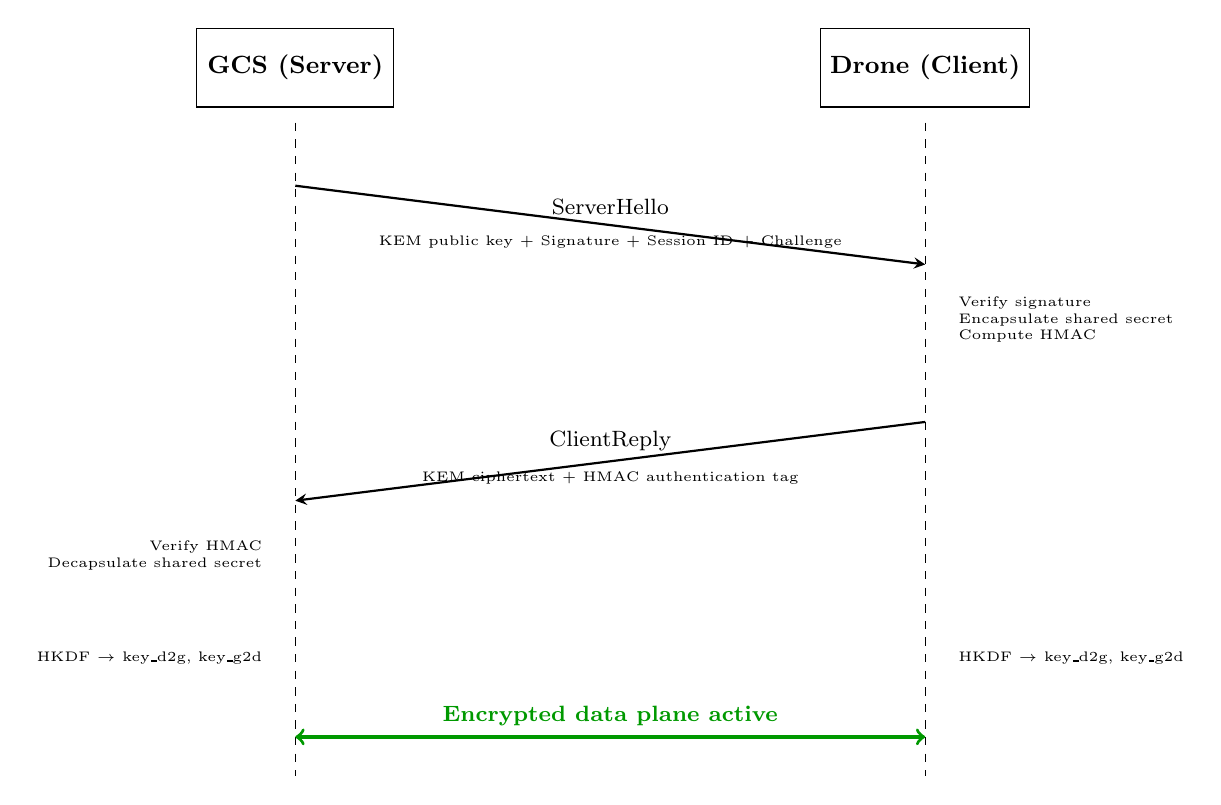
\begin{tikzpicture}[
    entity/.style={rectangle, draw, minimum width=2.5cm, minimum height=1cm, font=\small\bfseries},
    msg/.style={->, thick, >=stealth},
  ]
    \node[entity] (gcs) at (0,0) {GCS (Server)};
    \node[entity] (drone) at (8,0) {Drone (Client)};
    
    % Timeline
    \draw[dashed] (0,-0.7) -- (0,-9);
    \draw[dashed] (8,-0.7) -- (8,-9);
    
    % Message 1: ServerHello
    \draw[msg] (0,-1.5) -- node[above, font=\footnotesize] {ServerHello} node[below, font=\tiny] {KEM public key + Signature + Session ID + Challenge} (8,-2.5);
    
    % Drone processing
    \node[font=\tiny, right, align=left] at (8.3,-3.2) {Verify signature\\Encapsulate shared secret\\Compute HMAC};
    
    % Message 2: ClientReply  
    \draw[msg] (8,-4.5) -- node[above, font=\footnotesize] {ClientReply} node[below, font=\tiny] {KEM ciphertext + HMAC authentication tag} (0,-5.5);
    
    % GCS processing
    \node[font=\tiny, left, align=right] at (-0.3,-6.2) {Verify HMAC\\Decapsulate shared secret};
    
    % Key derivation
    \node[font=\tiny, left, align=right] at (-0.3,-7.5) {HKDF $\to$ key\_d2g, key\_g2d};
    \node[font=\tiny, right, align=left] at (8.3,-7.5) {HKDF $\to$ key\_d2g, key\_g2d};
    
    % Done
    \draw[<->, very thick, green!60!black] (0,-8.5) -- node[above, font=\footnotesize\bfseries] {Encrypted data plane active} (8,-8.5);
  \end{tikzpicture}
  \caption{The two-message PQC handshake protocol.}
  \label{fig:handshake-protocol}
\end{figure}

% ────────────────────────────────────────────────────────────────────────────
\section{Step 1: GCS Builds the ServerHello}
\label{sec:hs-server-hello}

The GCS (server) performs the following operations:

\begin{enumerate}
  \item \textbf{Generate KEM key pair:}
  \begin{lstlisting}[style=python, caption={KEM key generation}]
kem_obj = KeyEncapsulation("ML-KEM-768")
kem_pub = kem_obj.generate_keypair()
  \end{lstlisting}
  This produces a fresh ephemeral KEM key pair. The public key (\texttt{kem\_pub}) will be sent to the drone; the secret key is retained in \texttt{kem\_obj}.
  
  \item \textbf{Generate session ID:} 8 random bytes ($= 2^{64}$ possible values), uniquely identifying this session.
  
  \item \textbf{Generate challenge nonce:} 8 random bytes for freshness.
  
  \item \textbf{Construct transcript:} Concatenate all handshake data into a single byte string:
  \begin{equation}
    T = \text{version} \,\|\, \texttt{"pq-drone-gcs:v1"} \,\|\, \text{session\_id} \,\|\, \text{kem\_name} \,\|\, \text{sig\_name} \,\|\, \text{kem\_pub} \,\|\, \text{challenge}
  \end{equation}
  
  \item \textbf{Sign the transcript:} Using the GCS's long-term signature private key:
  \begin{lstlisting}[style=python, caption={Transcript signing}]
signature = server_sig_obj.sign(transcript)
  \end{lstlisting}
  
  \item \textbf{Serialize and send:} Pack all fields with length prefixes and send over TCP:
  \begin{equation}
    \text{ServerHello} = \text{version}(1) \,\|\, \text{kem\_name}(2+n) \,\|\, \text{sig\_name}(2+n) \,\|\, \text{session\_id}(8) \,\|\, \text{challenge}(8) \,\|\, \text{kem\_pub}(4+n) \,\|\, \text{signature}(2+n)
  \end{equation}
\end{enumerate}

\begin{securitynote}
The wire version byte is included as the \textbf{first byte of the transcript} before signing. This prevents a downgrade attack where an attacker strips newer security features by claiming an older protocol version. The signature covers the version, so tampering is detected.
\end{securitynote}

% ────────────────────────────────────────────────────────────────────────────
\section{Step 2: Drone Parses and Verifies the ServerHello}
\label{sec:hs-verify}

The drone receives the ServerHello and performs:

\begin{enumerate}
  \item \textbf{Parse the wire format:} Extract all fields using length prefixes. If parsing fails, raise \texttt{HandshakeFormatError}.
  
  \item \textbf{Reconstruct the transcript:} Using the same formula as the GCS.
  
  \item \textbf{Verify the digital signature:} Using the GCS's \textbf{pre-installed public key}:
  \begin{lstlisting}[style=python, caption={Signature verification}]
sig = Signature(sig_name)
if not sig.verify(transcript, signature, server_sig_pub):
    raise HandshakeVerifyError("bad signature")
  \end{lstlisting}
  If verification fails, the handshake aborts immediately. There is \textbf{no fallback}---this is deliberate.
  
  \item \textbf{Check suite consistency:} The drone verifies that the negotiated KEM and signature algorithms match what it expected. If they differ, it raises a \texttt{HandshakeVerifyError} indicating a potential downgrade attack.
\end{enumerate}

\begin{keyinsight}
The GCS's public signature key must be pre-installed on the drone \textbf{before deployment}. This is analogous to certificate pinning in TLS: the drone trusts exactly one GCS public key. If an attacker compromises the WiFi and tries a man-in-the-middle attack, they cannot produce a valid signature without the GCS's private key.
\end{keyinsight}

% ────────────────────────────────────────────────────────────────────────────
\section{Step 3: Drone Encapsulates and Authenticates}
\label{sec:hs-encap}

After verifying the ServerHello, the drone:

\begin{enumerate}
  \item \textbf{KEM Encapsulation:}
  \begin{lstlisting}[style=python, caption={KEM encapsulation}]
kem_ct, shared_secret = kem.encap_secret(server_hello.kem_pub)
  \end{lstlisting}
  This produces:
  \begin{itemize}
    \item \texttt{kem\_ct}: The KEM ciphertext (sent to GCS).
    \item \texttt{shared\_secret}: The raw shared secret (kept locally, 32 bytes).
  \end{itemize}
  
  \item \textbf{Drone HMAC authentication:}
  \begin{lstlisting}[style=python, caption={Drone authentication via HMAC}]
tag = hmac.new(psk_bytes, hello_wire, hashlib.sha256).digest()
  \end{lstlisting}
  The drone computes an HMAC-SHA256 over the \textbf{entire raw ServerHello wire bytes} using the pre-shared key. This proves the drone's identity to the GCS.
  
  \item \textbf{Send ClientReply:}
  \begin{equation}
    \text{ClientReply} = \text{len}(\text{kem\_ct})(4) \,\|\, \text{kem\_ct} \,\|\, \text{HMAC tag}(32)
  \end{equation}
\end{enumerate}

\begin{designdecision}
The drone authenticates via HMAC (symmetric) rather than a digital signature (asymmetric) to avoid deploying a second signature key pair on the drone. This simplifies key management: only the GCS needs a signature key pair; the drone only needs the GCS's public key and the shared PSK.
\end{designdecision}

% ────────────────────────────────────────────────────────────────────────────
\section{Step 4: GCS Verifies and Decapsulates}
\label{sec:hs-decap}

The GCS receives the ClientReply and:

\begin{enumerate}
  \item \textbf{Verify HMAC:} Recompute the expected HMAC using the same PSK and the ServerHello wire bytes, then compare using constant-time comparison (\funcname{hmac.compare\_digest}):
  \begin{lstlisting}[style=python, caption={HMAC verification on GCS}]
expected = hmac.new(psk_bytes, hello_wire, hashlib.sha256).digest()
if not hmac.compare_digest(tag, expected):
    raise HandshakeVerifyError("drone authentication failed")
  \end{lstlisting}
  If verification fails, the GCS logs the attempt (including the peer IP) and aborts.
  
  \item \textbf{KEM Decapsulation:}
  \begin{lstlisting}[style=python, caption={KEM decapsulation}]
shared_secret = kem_obj.decap_secret(kem_ct)
  \end{lstlisting}
  Using the ephemeral secret key retained from Step~1, the GCS recovers the same shared secret that the drone derived.
\end{enumerate}

\begin{securitynote}
The HMAC comparison uses \funcname{hmac.compare\_digest()}, which runs in constant time regardless of where the first mismatch occurs. This prevents timing side-channel attacks, where an attacker could learn the correct HMAC value one byte at a time by measuring response latency.
\end{securitynote}

% ────────────────────────────────────────────────────────────────────────────
\section{Step 5: Key Derivation}
\label{sec:hs-kdf}

Both sides now have the same \texttt{shared\_secret}. They independently derive the transport keys using HKDF-SHA256:

\begin{lstlisting}[style=python, caption={HKDF key derivation (both sides execute identically)}]
info = b"pq-drone-gcs:kdf:v1|" + session_id 
       + b"|" + kem_name + b"|" + sig_name
hkdf = HKDF(algorithm=SHA256(), length=64,
             salt=b"pq-drone-gcs|hkdf|v1", info=info)
okm = hkdf.derive(shared_secret)  # 64 output bytes
key_d2g = okm[:32]    # drone-to-GCS encryption key
key_g2d = okm[32:64]  # GCS-to-drone encryption key
\end{lstlisting}

\begin{description}
  \item[\texttt{key\_d2g}:] The 256-bit key the drone uses to encrypt and the GCS uses to decrypt.
  \item[\texttt{key\_g2d}:] The 256-bit key the GCS uses to encrypt and the drone uses to decrypt.
\end{description}

\begin{keyinsight}
Two separate keys are derived---one for each direction. This is a standard security practice: if key\_d2g were somehow compromised, traffic from GCS to drone (encrypted with key\_g2d) would still be secure. The HKDF \texttt{info} parameter includes the session ID, KEM name, and signature name for domain separation.
\end{keyinsight}

% ────────────────────────────────────────────────────────────────────────────
\section{Handshake Metrics}
\label{sec:hs-metrics}

Every handshake operation is timed with nanosecond precision using \funcname{time.perf\_counter\_ns()}:

\begin{table}[htbp]
  \centering
  \caption{Handshake timing metrics collected.}
  \label{tab:handshake-metrics}
  \small
  \begin{tabular}{lp{8cm}}
    \toprule
    \textbf{Metric} & \textbf{Description} \\
    \midrule
    \texttt{kem\_keygen\_ns}        & Time to generate the KEM key pair \\
    \texttt{kem\_encap\_ns}         & Time for the drone to encapsulate the shared secret \\
    \texttt{kem\_decap\_ns}         & Time for the GCS to decapsulate the shared secret \\
    \texttt{sig\_sign\_ns}          & Time to sign the transcript \\
    \texttt{sig\_verify\_ns}        & Time to verify the signature \\
    \texttt{handshake\_total\_ns}   & Wall-clock time for the entire handshake \\
    \texttt{public\_key\_bytes}     & Size of the KEM public key \\
    \texttt{ciphertext\_bytes}      & Size of the KEM ciphertext \\
    \texttt{signature\_bytes}       & Size of the digital signature \\
    \texttt{server\_hello\_bytes}   & Total size of the ServerHello wire message \\
    \bottomrule
  \end{tabular}
\end{table}

These metrics are critical for benchmarking: they reveal the true cost of each post-quantum algorithm in a real network round-trip.

\begin{implementationnote}
Both \funcname{time.perf\_counter\_ns()} (monotonic, high-resolution, no system clock drift) and \funcname{time.time\_ns()} (wall-clock, for correlating with external events) are recorded. The performance counter is used for benchmarking; the wall clock is used for timeline analysis.
\end{implementationnote}

% ────────────────────────────────────────────────────────────────────────────
\section{Error Handling}
\label{sec:hs-errors}

The handshake uses a hierarchy of specific exceptions:

\begin{description}
  \item[\texttt{HandshakeFormatError}:] Malformed wire data (bad lengths, truncated messages). Indicates a protocol error or network corruption.
  \item[\texttt{HandshakeVerifyError}:] Cryptographic verification failure (bad signature, bad HMAC, suite mismatch). Indicates an attack or misconfiguration.
  \item[\texttt{HandshakeError}:] General handshake failure (OQS unavailable, encapsulation failed). Indicates a runtime problem.
\end{description}

All three exceptions abort the handshake. There is no retry logic within the handshake itself; the caller (the proxy engine or scheduler) decides whether to retry.

% ────────────────────────────────────────────────────────────────────────────
\section{Cryptographic Key Lifecycle}
\label{sec:hs-key-lifecycle}

A session key in this system passes through six distinct phases.
Understanding the complete lifecycle is essential for reasoning about
the system's security properties---and its limitations.

\subsection{Phase 1: Key Generation (Handshake)}

During the handshake, the GCS calls \funcname{KEM.keygen()} to produce
an ephemeral key pair $(pk, sk)$.  Both keys exist only in process
memory; they are never written to disk.  The public key $pk$ is
transmitted to the drone in the ServerHello message; the secret key $sk$
is retained for decapsulation.

\subsection{Phase 2: Key Derivation (HKDF)}

After the KEM shared secret is established (via
\funcname{encapsulate}/\funcname{decapsulate}), both sides derive two
32-byte transport keys using HKDF-SHA256 with domain-separated
\texttt{info} and \texttt{salt} parameters
(Section~\ref{sec:hs-kdf}).  The raw KEM shared secret is \emph{not
used directly} for encryption---it is consumed solely as input keying
material (IKM) for the KDF.

\begin{securitynote}
After key derivation completes, the KEM shared secret, the KEM secret
key, and any intermediate HKDF state are no longer needed.  In the
current Python implementation, they become eligible for garbage
collection but are \textbf{not explicitly zeroised}.  Python's memory
model does not guarantee immediate overwrite of deallocated objects.
A production hardening step would be to use \texttt{ctypes.memset}
or a secure-memory library to overwrite sensitive buffers before
releasing them.
\end{securitynote}

\subsection{Phase 3: Active Use (AEAD Encryption)}

The derived keys (\texttt{key\_d2g} and \texttt{key\_g2d}) are
installed in the \classname{Sender} and \classname{Receiver}
dataclasses (Chapter~\ref{ch:aead}).  From this point, every MAVLink
datagram is encrypted with an AEAD algorithm using the key and a
deterministic nonce derived from the epoch and monotonic sequence
number.

During active use:
\begin{itemize}
  \item The sequence number increments strictly monotonically.
  \item The epoch byte remains constant (zero for the initial handshake).
  \item Both keys reside in Python process memory for the duration
        of the suite interval (typically 110~seconds in benchmark mode).
\end{itemize}

\subsection{Phase 4: Rekey (Suite Rotation)}

When the scheduling policy signals a suite change
(\texttt{NEXT\_SUITE}), the system performs a coordinated rekey:

\begin{enumerate}
  \item The scheduler sends \texttt{stop\_suite} to the GCS via the
        control channel.
  \item Both sides stop their proxy subprocesses (which destroys the
        in-memory keys when the process exits).
  \item A new handshake is performed for the next suite, generating
        entirely fresh KEM keypairs and deriving new transport keys.
  \item The new proxy processes start with the new keys.
\end{enumerate}

Within a single proxy session (without suite change), the
\funcname{bump\_epoch()} mechanism allows in-place epoch rotation:
the epoch byte increments and the sequence counter resets to zero,
providing fresh nonces under the same key material.  The epoch is
limited to 0--255; wrapping from 255 to 0 is \textbf{forbidden}---a
new full handshake must be performed before the epoch exhausts.

\begin{keyinsight}
Each suite rotation is a ``hard rekey'': the old proxy process
terminates (destroying all key material in its address space) and a new
process starts with fresh keys from a fresh handshake.  This provides
strong key separation between suites---there is no key material shared
across suite boundaries.
\end{keyinsight}

\subsection{Phase 5: Key Destruction (Normal Termination)}

On normal termination, the \classname{ManagedProcess} framework sends
\texttt{SIGTERM} (Linux) or \texttt{TerminateProcess} (Windows) to the
proxy subprocess.  When the process exits:

\begin{itemize}
  \item The Python garbage collector releases all objects, including
        the \texttt{bytes} objects holding key material.
  \item On Linux, the kernel reclaims the process's virtual memory
        pages.  On Windows, the process handle is closed and memory is
        freed.
  \item The key material is \textbf{not explicitly zeroised} before
        process exit.  The operating system's memory reclamation
        provides implicit cleanup, but a memory forensics tool running
        before page reuse could theoretically recover the keys.
\end{itemize}

\subsection{Phase 6: Crash Recovery}

If the proxy or scheduler process crashes unexpectedly:

\begin{enumerate}
  \item \textbf{Linux}: The \texttt{PDEATHSIG} mechanism delivers
        \texttt{SIGTERM} to orphaned child processes, causing them to
        exit (and releasing their key material).
  \item \textbf{Windows}: The Win32 Job Object terminates all
        children when the parent process exits.
  \item The crashed session's keys are irrecoverably lost (there is
        no persistent key storage).
  \item Recovery requires a \textbf{full new handshake}, which
        generates entirely fresh key material.
  \item No session resumption is possible---the system does not cache
        KEM shared secrets or derived keys.
\end{enumerate}

\begin{securitynote}
The lack of key persistence is a \textbf{security feature} for a
research system: there is no file or database that could leak
accumulated session keys.  The downside is that every crash
requires a full PQC handshake, which for heavy KEMs like Classic
McEliece can take tens of seconds.
\end{securitynote}

% ────────────────────────────────────────────────────────────────────────────
\section{Summary}
\label{sec:hs-summary}

\begin{itemize}
  \item The handshake is a \textbf{two-message TCP protocol}: GCS sends ServerHello, drone sends ClientReply.
  \item The GCS authenticates via \textbf{digital signature} (post-quantum); the drone authenticates via \textbf{HMAC-SHA256} with a pre-shared key.
  \item The shared secret is established via \textbf{KEM encapsulation/decapsulation} (post-quantum).
  \item Two 256-bit transport keys are derived via \textbf{HKDF-SHA256} with full domain separation.
  \item Every primitive operation is timed at \textbf{nanosecond precision} for benchmarking.
  \item Suite mismatch detection prevents \textbf{downgrade attacks}.
  \item The wire version is signed to prevent \textbf{version rollback attacks}.
\end{itemize}
